\input{../header}
\usetikzlibrary{shapes.geometric}

\begin{document}
%


%\onehalfspacing
\allowdisplaybreaks
%##################################################################
\section{Related rates recipe}
A lot of calculus students find related rates (and applied optimization) particularly tricky, and here's why: \textit{there's no formula for doing them.} Every situation is a bit different, and what works in one case doesn't necessarily work in another.

There is, however, a \textit{recipe} (if I was feeling very fancy I would call it a \textit{heuristic} -- google it) that you can follow to think your way through related rates problems.

\begin{enumerate}[leftmargin=15pt]
    \item Draw three pictures.
    \begin{itemize}
        \item I mean it. If you don't draw \textit{three}, it's harder to see what's changing.
        \item Draw your pictures pretty big, or you'll have a hard time labeling in the next step.
    \end{itemize}
    \item Decide what quantities are \textit{changing} (variables) and what ones are \textit{staying the same} (constants).
    \begin{itemize}
        \item If something is changing, label it in your pictures with a letter.
        \item If something is staying the same, label it in your pictures with what number it is.
    \end{itemize}
    \item Write down what you know and what you want to know.
    \begin{itemize}
        \item Use good derivative grammar, \(\dfrac{d\square}{dt}\), to label any rates.
        \item Make a note of what things are \textit{always} true and what things are only true \textit{at an instant}.
    \end{itemize}
    \item Write down an equation relating the variables.
    \begin{itemize}
        \item Creativity! Geometry! Trigonometry! Other math you remember!
    \end{itemize}
    \item Find the derivative, \textit{\textbf{with respect to time!!}}, of both sides.
    \begin{itemize}
        \item Remember, all of your variables are secretly some weird function of time.
        \item You have now \textit{related} the \textit{rates}!
    \end{itemize}
    \item Substitute in the values you know; solve for the rate you want.

\end{enumerate}

\pagebreak

\section{Preview for 11/5: Draw three pictures}

In this preview, we're going to practice the first two-ish steps of this recipe. For each of the 7 situations below (notice that 4(a) and 4(b) are a bit different!):
\begin{itemize}
    \item (Step 1) draw three pictures, 
    \item (Step 2) label them with variables and constants.
\end{itemize}
    

\everymath{\displaystyle}
\begin{enumerate}[leftmargin=0pt]

\item Beer is often brewed in big tanks where the bottom is a circular cone pointing down (\underline{\href{https://thumb.wikimedia.org/wikipedia/commons/thumb/8/87/Cuves_de_fermentations.jpg/960px-Cuves_de_fermentations.jpg}{like this}}). We're going to just focus on the cone part; let's say that the top radius of the cone is 6 feet and the depth of the cone is 8 feet. 
If I am draining the liquid out of the tank at a rate of \underline{\phantom{??}} \(  \text{ ft}^3 / \text{ min}\) \ldots

\item A television camera is positioned 4000 feet away from the base of a rocket launching pad. As the rocket goes up, the camera has to tilt up to keep the rocket in frame. In addition, the auto-focus of the camera has to take into account the increasing distance between the camera and the rocket.

If the rocket goes up at a speed of \underline{\phantom{??}} ft / sec \ldots
\begin{itemize}
    \item Note that the rocket is relatively \textit{small} (only a couple hundred feet tall) when compared to how far away the camera is (almost a mile).
\end{itemize}

\item A skateboarder who is 6 feet tall rides past a 15 foot tall lamppost. As he gets further from the lamppost, his shadow gets longer. 

\begin{itemize}
    \item Note that the tip of his shadow is at the place where light from the lamp hits the ground after juuuust touching the top of his head.
\end{itemize}

\item 
\begin{multicols}{2}
A baseball diamond is a big square that is 90 feet on each side (see the diagram on the right). 

A batter standing at home plate hits a ball along the line connecting home plate and third base, and starts running toward first base, 
\underline{\href{https://www.youtube.com/watch?v=3tMKgfJBcAU}{like this}}. 
\vfill
\begin{center}
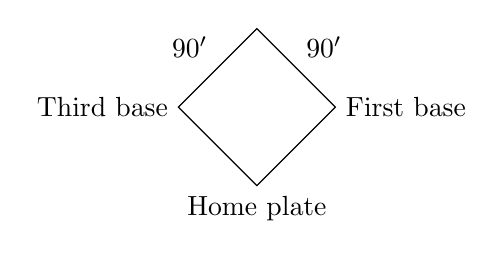
\begin{tikzpicture}
    \node[diamond, draw, minimum height=2cm, minimum width=2cm] (d) at (0, 0) {}; 
    \node[below] (home) at (d.south) {Home plate};
    \node[right] (1b) at (d.east) {First base};
    \node[left] (3b) at (d.west) {Third base};
    \node[above right] (1b2b) at (d.45) {$90'$};
    \node[above left] (2b3b) at (d.135) {$90'$};
\end{tikzpicture}
\end{center}
\end{multicols}
\begin{enumerate}
    \item Ignore the runner for now and just think about the ball: If the ball is going at a speed of \underline{\phantom{??}} (units?),
    how fast is the distance between the ball and first base changing?
    
    \item How fast is the distance between the ball and the runner changing?
\end{enumerate}

\item A boat is being pulled towards a dock using a long rope.  One end of the rope is attached to the boat 3 feet above the water; the other end is attached to a \underline{\href{https://www.dockboxes.com/site/wp-content/uploads/2022/12/8-Winch_CP.jpg}{winch}} (a machine that winds up rope) at a height of 10 feet above the water.

\item While Violet Beauregarde is at Willy Wonka's Chocolate Factory, she snatches some experimental gum against Wonka's warnings. Not yet perfected, the gum has the side effect of \href{https://www.youtube.com/watch?v=8Yqw_f26SvM}{expanding Violet into a giant spherical human blueberry}. If she expands at a rate of \underline{\phantom{??}} (units?)\ldots
\end{enumerate}
\end{document}